\documentclass{article}
\usepackage[table]{xcolor}
\usepackage[paper=letterpaper,left=1.2cm,right=1.2cm,top=1cm,bottom=1cm,includefoot]{geometry}
\usepackage{tabularx}
\usepackage{multirow}
\usepackage{hyperref}
\usepackage{hhline}
\usepackage{amsmath}
\usepackage{enumitem}
\usepackage{pgfgantt}
\usepackage{graphicx}   \graphicspath{{img/}}
\usepackage{subfigure}
\usepackage{subcaption}

\usepackage[spanish]{babel}
\usepackage[utf8]{inputenc}


%%% Comente/Descomente las siguientes lineas para cambiar la fuente del texto
\usepackage{DejaVuSans}
\renewcommand*\familydefault{\sfdefault}
% \usepackage{sansmath}
% \sansmath

\pagestyle{empty}

\definecolor{tcc}{RGB}{217,217,217} % Table cell color

\renewcommand\tabularxcolumn[1]{m{#1}}
\setlength{\arrayrulewidth}{0.5pt}
\renewcommand{\arraystretch}{2}

\renewcommand{\thesection}{\alph{section})}
\renewcommand{\thesubsection}{\alph{section}.\arabic{subsection}}

\renewcommand{\refname}{\vspace{-2ex}}

\begin{document}
	
	\noindent
	\begin{tabularx}{\textwidth}{|>{\columncolor{tcc}}m{5.7cm}|X|} \hline
		\textbf{Integrantes:} & \textbf{Felipe Andre Ahumada Silva, Martin Alberto Garrido Briano, Nelson Eduardo Gallegos Pastén}
		\\ \hline
		\textbf{Título del proyecto:} & \textbf{Simulación del movimiento de las particulas en un plasma electrostático}
		\\ \hline
		\textbf{Asignatura:} & \textbf{Física Computacional II (510240)} \newline Departamento de Física \newline Facultad de Ciencias Físicas y Matemáticas \newline Universidad de Concepción
		\\ \hline
		\textbf{Profesor:} & Dr. Roberto E. Navarro
		\\ \hline
		\textbf{Ayudante:} & Lorena Sepúlveda
		\\ \hline
		
	\end{tabularx}
	
	
	\bigskip
	
	\noindent\begin{tabularx}{\textwidth}{|>{\columncolor{tcc}}X|}
		\hline
		En esta sección, explique en detalle los siguientes aspectos:
		\begin{enumerate}[label={\alph*)},nosep]
			\item Descripción breve de la propuesta.
			\item Objetivos de trabajo.
			\item Metodología de trabajo y herramientas disponibles para cumplir los objetivos.
			\item Resultados.
			\item Conclusión.
		\end{enumerate}
		
		\medskip
		
		Número máximo de palabras del documento: \textbf{1500 palabras}.\\
		\hline
	\end{tabularx}
	
	%%%%%%%%%%%%%%%%%%%%%%%%%%%%%%%%%%%%%%%%%%%%%%%%%%%%%%%%%%%%%%%%%%%%%%%%%%%%%%%%
	\section*{Propuesta de proyecto:}
	
		Nos planteamos simular el movimiento de las partículas dentro de un plasma electrostático en una dimensión, para esto vamos a utilizar el método PIC (Particle in cell), el cual es una técnica comúnmente usada para simular plasmas. A grandes rasgos esta metodología consiste de definir el espacio (en nuestro caso unidimensional) donde se distribuyen aleatoriamente las partículas y dividirlo en secciones discretas llamadas celdas. En cada celda se calculará la densidad de carga y luego el campo eléctrico a partir de la solución de la ecuación de Maxwell en una dimensión,
	\begin{equation}
		\nabla \cdot \mathbf{E} = \frac{dE}{dx} = \rho,
	\end{equation}
	ya calculado el campo eléctrico se obtendrá la ecuación de movimiento para cada partícula.
	
	%%%%%%%%%%%%%%%%%%%%%%%%%%%%%%%%%%%%%%%%%%%%%%%%%%%%%%%%%%%%%%%%%%%%%%%%%%%%%%%%
	\section{Objetivos de trabajo}
	
	\subsection{Objetivo general}
	
	Simular el movimiento de partículas en un plasma electrostático
	
	\subsection{Objetivos específicos}
	\begin{enumerate}
		\item Escribir las formulas necesarias para el desarrollo del proyecto.
		\item En base a estas formulas crear un código que realice nuestra simulación.
		\item Ya descrito el movimiento del las partículas, simular el fenomeno llamado 'inestabilidad two-stream'.
	\end{enumerate}
	
	\section{Metodología}
	
	\begin{enumerate}
		\item Se verificarán las condiciones de borde.
		\item Calcularemos la densidad de carga en cada celda.
		\item Se estimará el campo eléctrico para cada celda.
		\item Se resolverá computacionalmente las ecuaciones de movimiento para cada partícula, actualizando las velocidades y moviendo las partículas a una nueva ubicación.
	\end{enumerate}
	
	\section{Resultados}
	
	Se ha podido describir correctamente el movimiento de partículas en una dimensión , además de poder visibilizar el fenomeno de la inestabilidad two-stream.
	
	\begin{figure}[h]
		\begin{subfigure}
			\centering
			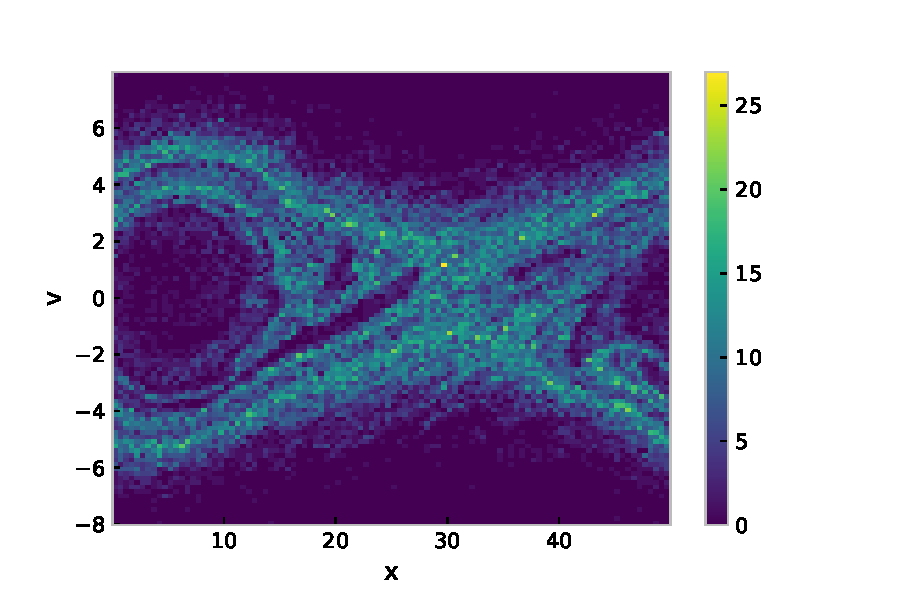
\includegraphics[width=.5\linewidth]{inestabilidad.pdf}
			\label{fig:sfig1}
		\end{subfigure}%
		\begin{subfigure}
			\centering
			\includegraphics[width=.5\linewidth]{particulas.pdf}
			\label{fig:particulas}
		\end{subfigure}
		\caption{Resultados}
		\label{fig:resultados}
	\end{figure}
	
	\section{Conclusión}
	
	Ya desarrollado el código en su totalidad se modificaron varias ideas vistas en un principio, en las condiciones iniciales, por ejemplo, utilizamos una gran cantidad de partículas, además de agregar que la velocidad tenga un comportamiento sinusoidal, cuando en un principio utilizabamos pocas partículas para describir el movimiento y no se consideraba el espacio de fase finalmente realizado.\\
	
	En definitiva, el método PIC nos dio un buen resultado para poder simular el movimiento de las partículas, además nuestro código muestra una buena eficiencia al momento de trabajar con altas cantidades de partículas, lo cual es muy útil para simular este tipo de sistemas.
	
	Surgieron varios problemas a la hora de calcular la densidad de partículas y esto fue principalmente, por no normalizar los electrones, de esta forma en un próximo proyecto lo ideal sería revisar el orden de magnitud de los datos utilizados.
	
	
	% lista de referencias guardadas en referencias.bib
	\bibliographystyle{amsplain}
	\bibliography{referencias}
	
\end{document}
